%\documentclass[conference]{IEEEtran}
%\documentclass[journal,onecolumn,draftclsnofoot,]{IEEEtran}
\documentclass[12pt]{report}
%\documentclass[conference]{IEEEtran}
%\documentclass{acm_proc_article-sp}
%%%% ADDED -- PPD --- START
\usepackage{graphicx}
\usepackage{float}
\usepackage{bbding}
\usepackage{fancyvrb}
\usepackage{color,soul}
\usepackage{graphicx}
\usepackage{float}
\usepackage{bbding}
\usepackage{enumerate}
\usepackage{color,soul}
\usepackage{graphicx}
\usepackage{float}
\usepackage{bbding}
\usepackage{amsmath}
\usepackage{xcolor}
%\usepackage{hyperref}
\usepackage{colortbl}
\usepackage{fancybox}
\usepackage{amssymb}
\usepackage{pdfpages}
\usepackage{tikz}
\usepackage{array}
\usepackage{multirow}
%\usepackage{subcaption}
\usepackage{capt-of}
\usepackage{color,soul}
\usetikzlibrary{fit,shapes.geometric}
\usepackage{latexsym}
\usepackage{hyperref}
\usepackage{graphicx}
\usepackage{subcaption}
\usepackage[utf8]{inputenc}

%\usepackage[a4paper, lmargin=0.8in, rmargin=0.8in, tmargin=0.6in, bmargin=0.6in]{geometry}
\renewcommand{\thesection}{\Roman{section}} 
\usepackage[lmargin=1in, rmargin=1in, tmargin=1in, bmargin=1in]{geometry}

%\usepackage{enumitem}
%\usepackage[inline]{enumerate}
%\usepackage[inline]{enumitem}
%%%% ADDED -- PPD --- END
\begin{document}
	\thispagestyle{empty}
	\input{epsf}
	\begin{center}
		{\Huge \bf Measurements in physical optics}
	\end{center}
	\vspace{0.5cm}
	{\centering {\Large Electromagnetism and Optics Laboratory}\par}
	{\centering {\Large PH39008}\par}
	
	\vspace{5.5cm}
	
	{\centering \textbf{\Large Vinit Kumar Singh}\par}
	{\centering \large Roll No: 16PH20036 \par}
	{\centering \large \em vinitsingh911@gmail.com \par}
	\vspace{0.5cm}
	
	\begin{figure}[h]
		\centering
		
\includegraphics[height=3cm,width=3cm]{IIT_Logo.png}
	\end{figure}
	
	\begin{center}
		{\textbf{Date: 15.01.2019} \\
			\textbf{Department: Physics} \\
			\textbf{Indian Institute of Technology, Kharagpur,}\\
			\textbf {WB 721302, India}\\
			
		}
	\end{center}
	\newpage
	\tableofcontents
	
	\newpage
	\chapter{Introduction and motivation}
	\section{Summary of experiments performed}
	\begin{enumerate}
		\item Using a Fabry Perot Interferometer and a LASER we measure:-
		\begin{itemize}
			\item the wavelength of laser light.
			\item the separation between two mirrors.
			\item the free spectral range.
		\end{itemize}
		\item Using a Fabry Perot Interferometer and a sodium vapour lamp we:-
		\begin{itemize}
			\item determine the wavelength of sodium light.
			\item measure the difference in the wavelengths between the D1 and D2 lines of Na.
			\item Find the fractional order at the centre of the fringe system.
		\end{itemize}
		\item Using Michelson Interferometer and a LASER we measure:-
		\begin{itemize}
			\item the wavelength of laser light. 
			\item the refractive index of a given glass plate.
		\end{itemize}
		\item Using Michelson Interferometer and a sodium vapour lamp we:-
		\begin{itemize}
			\item determine the wavelength of sodium light.
			\item determine the difference in the wavelengths between the D1 and D2 lines of Na.
			\item measure the thickness of givem mica sheet.
		\end{itemize}
	\end{enumerate}
	
	\chapter{Experimental set-ups and relevant theory}
	\section{Fabry Perot Interferometer with laser }
	\textsc{\large{Apparatus:}}
	\begin{itemize}
		\item Optical Breadboard
		\item Diode Laser
		\item Laser mount
		\item Etalon
		\item Screen
		\item Detector
		%\item Counter
	\end{itemize}
	\textsc{\large{Theory: }}
	\begin{figure}[h]
		\centering
		\includegraphics{1.png}
	\end{figure}
	Fabry – Perot Interferometer consists of two plane mirrors (M1, M2) mounted accurately parallel to one another, with a spacing d between them. This arrangement is called Fabry – Perot etalon. The inner surfaces of mirrors are coated with partially transparent films of high reflectivity. The plates themselves are made slightly prismatic in order to avoid disturbing effects due to reflections at the outer uncoated surfaces.\\\\
	Determination of wavelength of LASER light:\\
	For mth order bright ring at the centre we have,
	$$2d = m\lambda$$
	$$2(d + \frac{\lambda}{2}) = m\lambda$$
	each time d increases by $\lambda$/2, one fringe crosses the center of view. If the total displacement of the movable mirror be ($y_2-y_1$) for N bright rings to cross the center, we have,
	$$0.5N\lambda = y_2 - y_1$$
	$$\lambda = \frac{2(y_2-y_1)}{N} $$
	Determination of distance between the plates of Fabry Perot Etalon (d):\\
	Let $X_m$ be the distance of $m^th$ order bright fringe from the central one, D is the distance between the source and the screen.
	$$tan\theta_m = \frac{X_m}{D}-\theta_m$$ when D is very large
	Hence,
	$$cos\theta_m = \frac{1}{1-\frac{X^2_m}{D^2}}$$
	For bright fringe we know the required condition is 
	$$ 2dcos\theta_m = m\lambda$$
	Hence,
	$$m = \frac{2d}{\lambda}[cos\theta_m - cos\theta_{m+1}]$$
	$$ = \frac{2d}{\lambda}\Big[\Big(\frac{1}{1-\frac{X^2_m}{D^2}}\Big)-\Big(\frac{1}{1-\frac{X^2_{m+1}}{D^2}}\Big)\Big]$$
	$$ = \frac{d}{D^2\lambda} X^2_n$$
	where $X^2_n = X^2_{m+n} - X^2_m$\\
	Therefore,
	$$ d = \frac{mD^2\lambda}{X^2_n} $$\\
	To measure the free spectral range(FSR)\\ 
	Free Spectral Range (FSR) is the spacing in optical frequency or wavelength between two successive reflected or transmitted optical intensity maxima or minima of an interferometer.\\
	\begin{center}
		FSR = c/2d
	\end{center}       
	d = distance of separation of two mirrors. Free Spectral Range is inversely proportional to plate reading d. So increase of resolving power obtained by increasing plate separation is accompanied by proportionate reduction of spectral range. 
	\begin{figure}[h!]
		\centering
		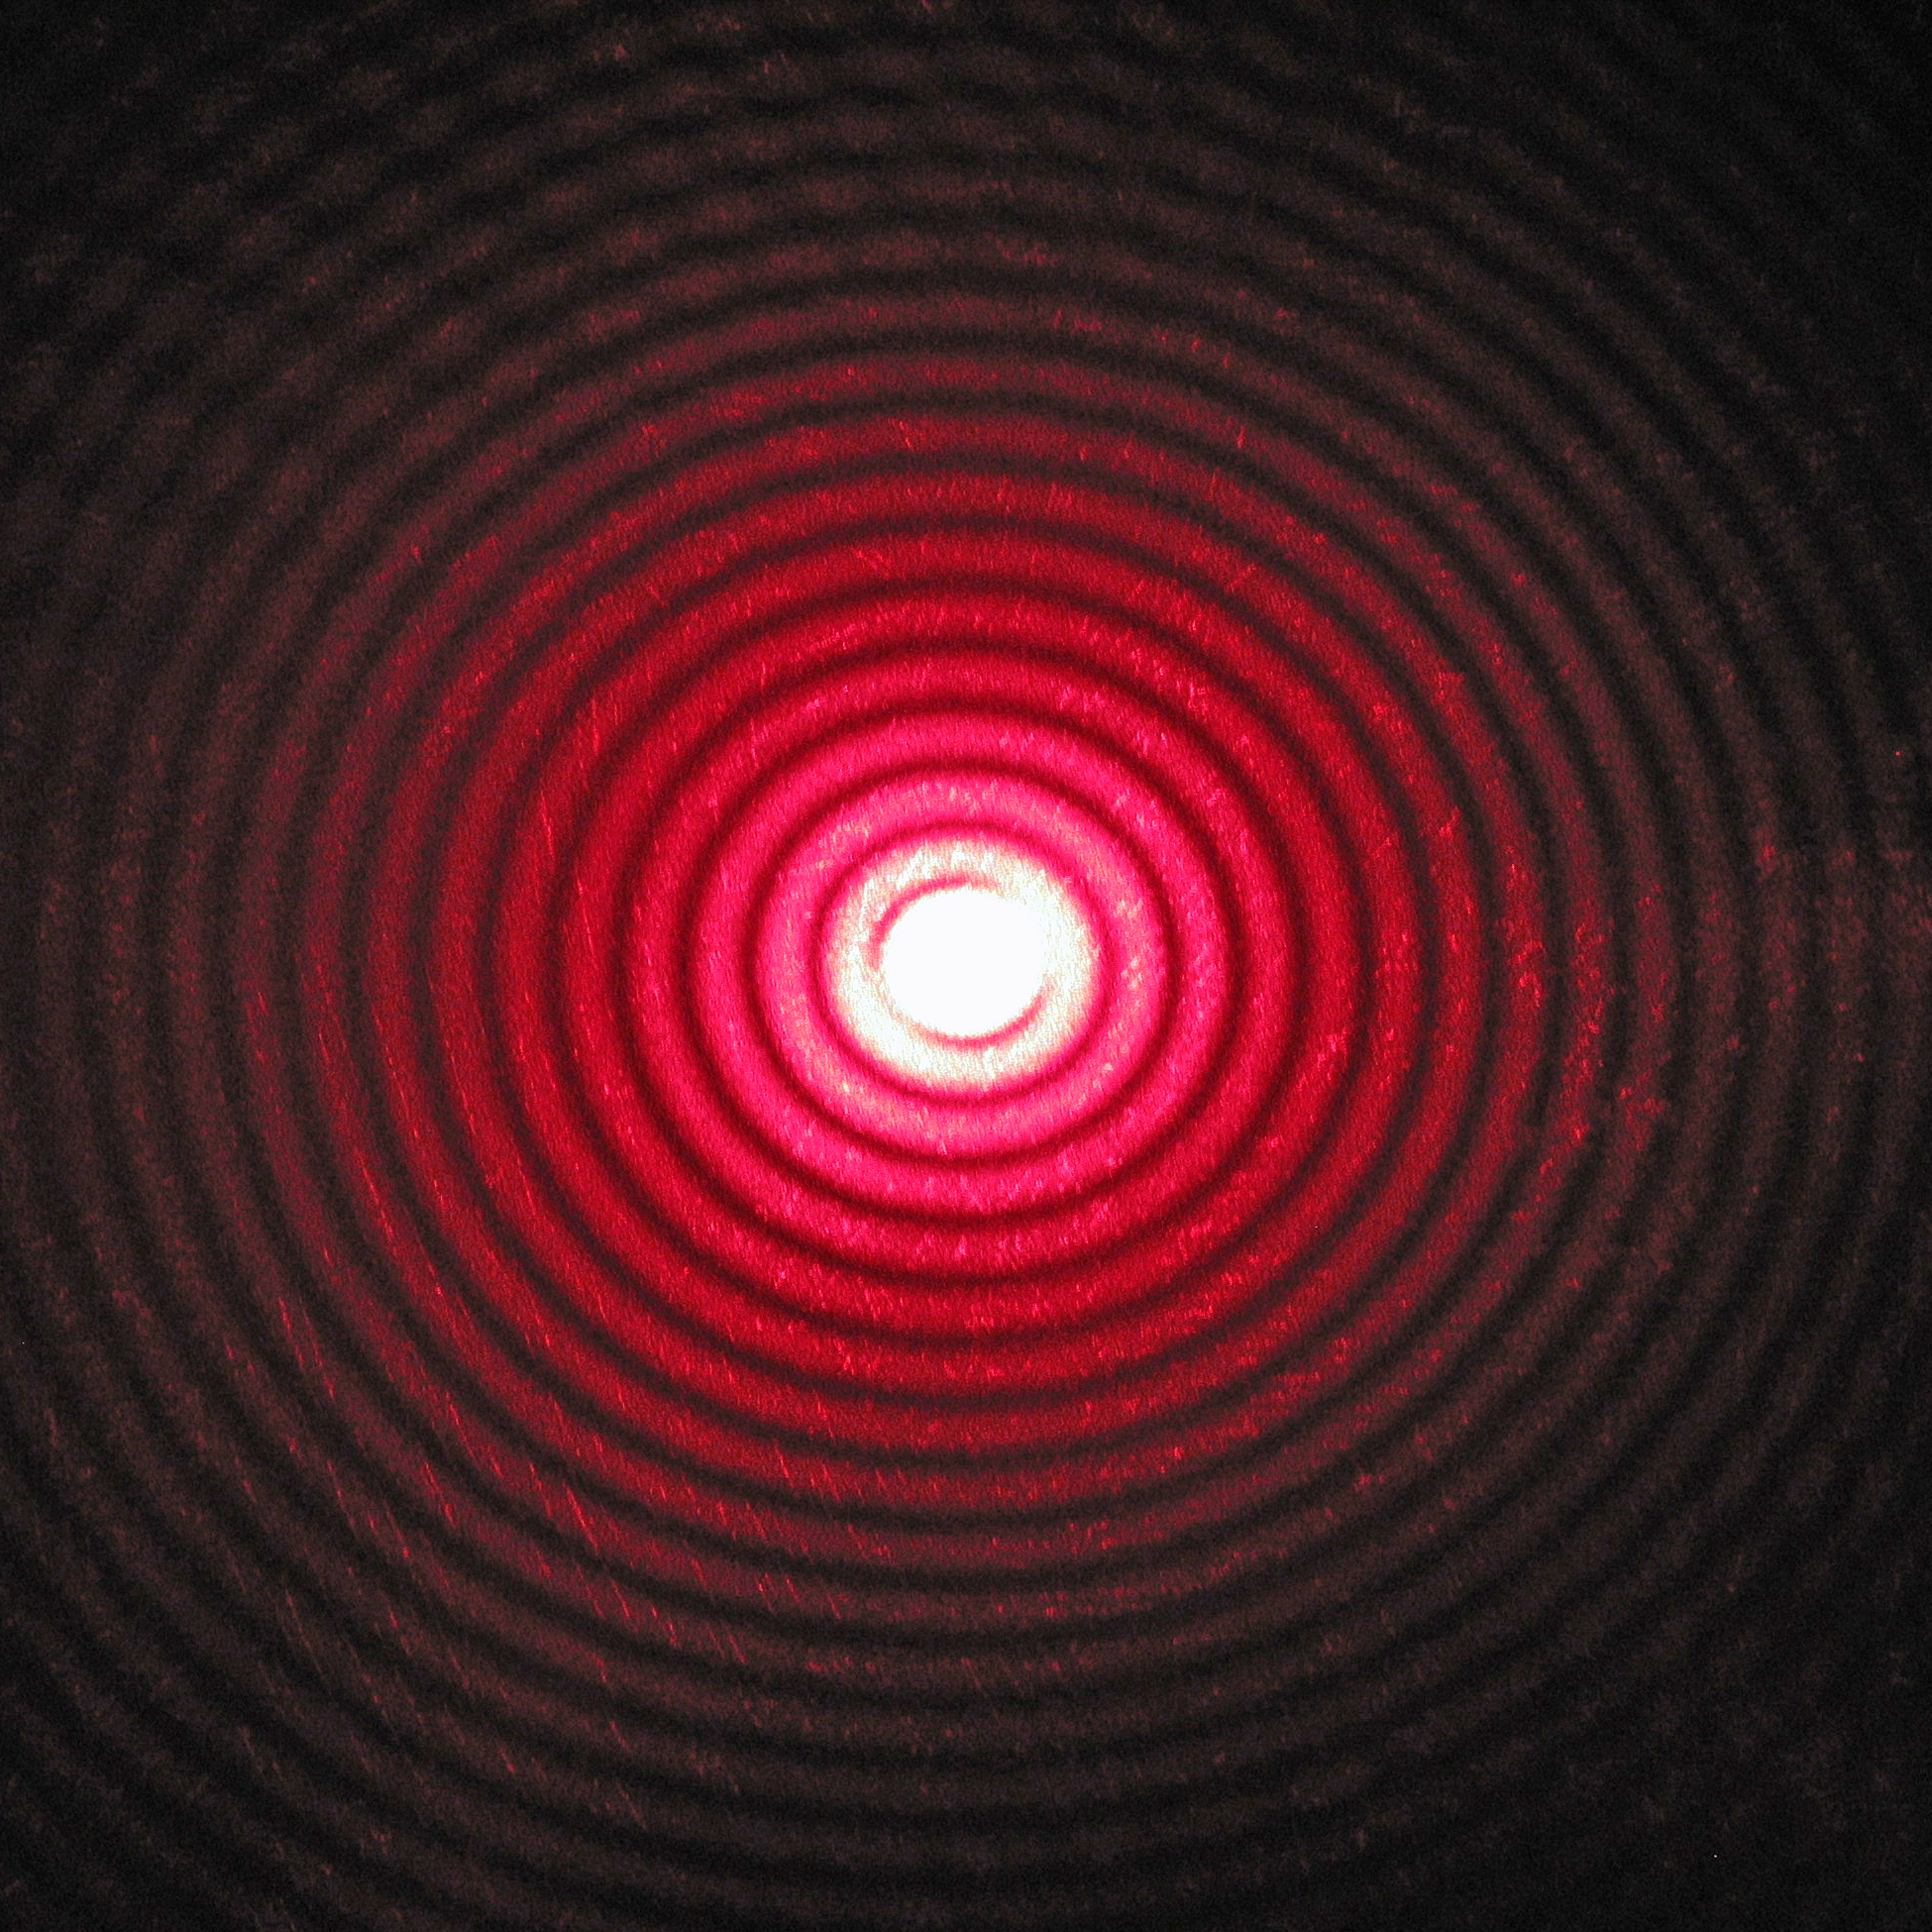
\includegraphics[width=0.4\textwidth]{5.png}
	\end{figure}
	\newpage
	\section{Fabry Perot Interferometer with Sodium Lamp}
	\textsc{\large{Apparatus: }}
	\begin{itemize}
		\item Fabry Perot Interferometer
		\item Sodium Vapour Lamp
		\item Very small circular aperture
	\end{itemize}
	\textsc{\large{Theory:}}
	\\
	\begin{center}
		\includegraphics{1.png}
	\end{center}
	It basically consists of two glass plates of which the inner surfaces are made plane, accurately parallel and thinly silvered. The outer surfaces (uncoated) are made to have a small angle away from the coated surfaces (helping to throw away the unwanted fringes formed due to multiple reflections in the plate itself. The thickness of the film (between the two plates) can be varied. Concentric circular fringes of equal inclination are obtained on the screen after multiple internal reflections between the plates.\\
	Determination of wavelength of Na light:\\For m th order bright ring at the centre we have,
	$$2d = m\lambda$$
	$$2(d + \frac{\lambda}{2}) = m\lambda$$
	each time d increases by $\lambda$/2, one fringe crosses the center of view. If the total displacement of the movable mirror be ($y_2-y_1$) for N bright rings to cross the center, we have,
	$$0.5N\lambda = y_2 - y_1$$
	$$\lambda = \frac{2(y_2-y_1)}{N} $$
	Determination of wavelength separation of Na lines (D1 and D2):\\The separation (d) between the plates is adjusted until the ring systems of two wavelength coincide. Under this condition concordance occurs. For first concordance\\
	$2d_1 = m_1\lambda_1 = \big(m_1+\frac{\lambda}{2}\big)\lambda_2$\\
	$m_1\rightarrow$ order of $\lambda_1$ at centre.\\
	For the next concordance,\\
	$2d_1 = m_2\lambda_1 = \big(m_2+\frac{\lambda}{2}\big)\lambda_2$\\
	$m_2\rightarrow$ order of $\lambda_1$ at centre.\\
	$2(d_2-d_1) = (m_2-m_1)\lambda_1 = (m_2-m_1)\lambda_2 + \lambda_2$\\
	$\rightarrow m_2-m_1 = \frac{\lambda_2}{\lambda_1-\lambda_2}$\\
	$\Delta\lambda = \lambda_1-\lambda_2 = \frac{\lambda_1\lambda_2}{2(d_2-d_1)} = \frac{\lambda^2_{av}}{2(d_2-d_1)} $\\
	Finding fractional order at the centre of the fringe system:\\The axis of the lens is usually normal to the plates, and the bright fringes, corresponding to integral values of m, are then circles with common centre at the focal point for normally transmitted light. At this point, m has max.value:\\
	$$m_0 = m_1 + e$$
	where $m_1$ is integral order of the innermost bright fringe, and e, having value less than unity  is the fractional order at the center. The angular radius $\theta_p$ of the $p^{th}$ bright fringe from the center, when $\theta_p$ is not too large is
	$$ \theta_p = \frac{1}{n}\sqrt{\frac{n'\lambda_0}{d}}\sqrt{p-1+e}$$
	when n=refractive index of the air outside the plates and n'=refractive index of the air between the plates. \\The diameter Dp of this fringe is then given by,
	$$D^2_p = (2f\theta_p)^2 = \frac{4n'\lambda_0f^2}{n^2d}(p-1+e)$$
	where f id the focal length of the lens
	\begin{figure}[h]
		\centering
		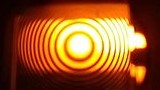
\includegraphics{4.png}
	\end{figure}
	\newpage
	\section{Michelson Interferometer with laser}
	
	\textsc{\large{Apparatus: }}
	\begin{itemize}
		\item Optical Breadboard
		\item Diode Laser
		\item Laser mount
		\item Beam-splitter mount
		\item Mirror mounts
		\item Screen
		\item Detector
		\item Counter
	\end{itemize}
	\textsc{\large{Theory:}}
	\\
	\includegraphics{27.png}\\
	$M_1$ and $M_2$ are two plane mirrors silvered on the front surfaces. They are mounted vertically on two translation stages placed at the sides of the optical platform. Screws are provided at the back of the holders, adjustment of which allows $M_1$ and $M_2$ to be tilted. $M_1$ can also be moved horizontally by a micrometer attached to the $M_1$ holder. BS is a 50\%-50\% beam-splitter, which is a planar glass plate slightly silvered on one side. It is mounted vertically and at an angle $45^o$ to the direction of incident light.
	When light from laser is allowed to fall on BS, one portion, beam A, is transmitted through BS to $M_2$ and the other, beam B is reflected by BS to $M_1$. Beam A returning from $M_2$ is reflected at the back of BS to reach the screen, and beam B after getting reflected from $M_1$ passes through BS to reach the screen.  If $\lambda$ is the wavelength of laser light and D is the change in the separation between the mirrors $M_1$ and $M_2$ that occurs for ‘n’ fringes to collapse or evolve then
	$$\lambda = \frac{2D}{n}$$
	The optical path lengths of one of the light paths will change if a glass plate is inserted into it. As the glass plate is rotated, the length of glass in the path will increase and therefore the number of wavelengths in that path will increase. This will change the interference pattern. The refractive index of the glass plate can be calculated from the number of interference fringes shifted during the rotation of the glass plate through some angle $\theta$. The refractive index of the glass plate is then given by:
	$$n_g = \frac{(2t-N\lambda)(1-cos\theta)}{2t(1-cos\theta)-N\lambda} $$
	Where, N = number of shifted fringes;  $\theta$ = the angle of rotation;  $\lambda$ = the wavelength of light used;  t = thickness of the glass plate.
	\newpage
	\section{Michelson Interferometer with Na Lamp} 
	
	\textsc{\large{Apparatus: }}
	\begin{itemize}
		\item Michelson Interferometer
		\item Sodium Vapour Lamp
		\item White Light source
		\item Mica Sheet 
	\end{itemize}
	\textsc{\large{Theory:}}
	\\
	\includegraphics{27.png}\\
	M$_1$ and M$_2$ are two plane mirrors silvered on the front surfaces. They are mounted vertically on two translation stages placed at the sides of the optical platform. Screws are provided at the back of the holders, adjustment of which allows M$_1$ and M$_2$ to be tilted. M$_1$ can also be moved horizontally by a micrometer attached to the M$_1$ holder. BS is a 50\%-50\% beam-splitter, which is a planar glass plate slightly silvered on one side. It is mounted vertically and at an angle 45$^o$ to the direction of incident light. When light from the lamp is allowed to fall on BS, one portion, beam A, is transmitted through BS to M$_2$ and the other, beam B is reflected by BS to M$_1$. Beam A returning from M$_2$ is reflected at the back of BS to reach the screen, and beam B after getting reflected from M$_1$ passes through BS to reach the screen.\\\\
	The average wavelength of Na light,
	$$ \lambda_{av} = \frac{2\Delta d}{\Delta n} $$
	where, $\Delta d = $ distance moved by M1\\
	\qquad $\Delta n = $ no. of fringes collapsed at the centre.\\\\
	The difference in wavelength of Na doublet (D1,D2) is
	$$ \Delta \lambda = \frac{\lambda^2_{av}}{2d}$$
	where, d = distance between 2 positions of maxima in coherent\\
	\qquad $\lambda_{av} =  $mean wavelength between positions of maximums.\\\\
	The relation between refractive index and thickness of mica sheet is
	$$ t = \frac{\Delta d}{\mu - 1}$$
	where, t = thickness of mica sheet\\
	\qquad $\mu = $refractive index of mica
	
	\chapter{Experimental results and analysis}
	
	\section{Fabry Perot Interferometer with Laser}
	\textbf{Calibrating the micrometer attached to the movable mirror M1.}\\
	The movable mirror mount is mounted on a translation stage. The micrometer shaft
	actuates a lever arm which pushes the translation stage carrying the mirror. To make
	proper measurements it is first necessary to obtain the calibration factor or reduction ratio
	R, which gives the correspondence between the distance d’ moved by the micrometer
	screw and the actual motion D of the mirror M1.
	Here 10 microns (= 0.01 mm) on the thimble of the micrometer (= 1 division) is equivalent
	to 35 microns on the translation stage, i.e., when we move one step on the micrometer, the
	mirror is moved 0.35 microns. Hence
	$$R=0.35/10=0.035$$
	Thus D in eq (1) becomes:
	$$D=0.035*d'$$
	\textbf{Determination wavelength of the laser light.}\\
	Least count of the micrometer attached to the movable mirror:-\\
	Value of 1 small division of the main scale = 1mm\\
	Pitch of the screw = P = 0.5mm\\
	Total number of divisions on the circular scale = N = 50\\
	Least count of micrometer = P/N = 0.5/50 = 0.01mm\\ \\
	\textbf{Data for the distance D moved by the movable mirror for number of fringes to evolve/collapse}
	\begin{center}
		\begin{tabular}{ |c|c|c|c|c| } 
			\hline
			No of fringes &Initial micrometer&Final micrometer& d (mm) & D (mm)\\
			appear/collapse (N)&reading (y1) &reading (y2)&(y2-y1)& =d*0.035\\
			\hline
			100 & 3.5  & 4.31 & 0.81 & 0.028 \\
			200 & 1.96 & 3.6  & 1.64 & 0.057 \\
			300 & 1.5  & 3.98 & 2.48 & 0.087 \\
			400 & 1.0    & 4.3  & 3.3  & 0.116 \\
			\hline
		\end{tabular}
		\\
	\end{center}
	\begin{figure}[h]
		\centering
		\includegraphics{FL1.png}
	\end{figure}
	Slope of the plot = 0.0291\\
	Wavelength of light = 581.7 nm\\ \\
	\textbf{Data to measure the diameter of the rings.}\\
	Taking m=0.
	\begin{center}
		\begin{tabular}{ |c|c|c| } 
			\hline
			Fringe No.&Value of Xm+n (mm)&$X_n^2 = X_{m+n}^2 - X_m^2(mm^2)$\\
			\hline
			0 & 0     & 0.00   \\
			1 & 3.4   & 11.56  \\
			2 & 5.3   & 28.09  \\
			3 & 6.81  & 46.38  \\
			4 & 8.18  & 66.91  \\
			5 & 10.05 & 101.00 \\
			6 & 10.94 & 119.68 \\                           
			\hline
		\end{tabular}
		\\
	\end{center}
	\begin{figure}[h]
		\centering
		\includegraphics{FL2.png}
	\end{figure}
	
	\newpage
	$$d=\frac{mD^2\lambda}{X_n^2}$$
	Distance between the source and the screen (D) = 55 cm.\\
	Slope of $X_n^2$ vs. n plot: 20.599 $mm^2$\\
	$d=\frac{D^2\lambda}{slope} = 8.54 mm$\\
	\textbf{Determination of the separation between two mirrors and FSR}
	\begin{center}
		\begin{tabular}{ |c|c|c|c|c| } 
			\hline
			Slope&Distance D&Wavelength of&Mirror Separation&FSR\\
			&&the source ($\lambda$)&$d=\frac{D^2\lambda}{slope} (mm)$&=$\frac{c}{2d}$\\
			\hline
			20.599 & 55 & 581.7 & 8.54 & 3.51$\times10^{10}$ Hz\\
			\hline
		\end{tabular}
		\\
	\end{center}
	
	
	\newpage
	\section{Fabry Perot Interferometer with Sodium Lamp}
	\textbf{Calibrating the micrometer attached to the movable mirror M1.}\\
	The movable mirror mount is mounted on a translation stage. The micrometer shaft
	actuates a lever arm which pushes the translation stage carrying the mirror. To make
	proper measurements it is first necessary to obtain the calibration factor or reduction ratio
	R, which gives the correspondence between the distance d’ moved by the micrometer
	screw and the actual motion D of the mirror M1.
	Here 10 microns (= 0.01 mm) on the thimble of the micrometer (= 1 division) is equivalent
	to 12 microns on the translation stage, i.e., when we move one step on the micrometer, the
	mirror is moved 0.12 microns. Hence
	$$R=0.12/10=0.012$$
	Thus D in eq (1) becomes:
	$$D=0.012*d'$$\\
	\textbf{Determination of the wavelength of the Sodium Lamp.}\\
	Smallest division of the linear scale= s = 0.5mm\\
	Pitch of the screw = p = 0.5mm\\
	Number of divisions on the circular scale = N = 50\\
	Least count of instrument = l.c. = p/N = 0.01mm\\
	Scaling factor for measuring displacement of the mirror : 0.012\\ \\
	\textbf{Data for the distance D moved by the movable mirror for number of fringes to evolve/collapse}
	\begin{center}
		\begin{tabular}{ |c|c|c|c|c| } 
			\hline
			No of fringes &Initial micrometer&Final micrometer& d (mm) & D ($\mu$m)\\
			appear/collapse (N)&reading (y1) &reading (y2)&(y2-y1)& =d*0.012\\
			\hline
			10 & 1.50 & 1.74 & 0.24 & 2.88  \\
			20 & 1.50 & 1.97 & 0.47 & 5.64  \\
			30 & 1.50 & 2.21 & 0.71 & 8.52  \\
			40 & 1.50 & 2.45 & 0.95 & 11.40 \\
			50 & 1.50 & 2.68 & 1.18 & 14.16 \\
			\hline
		\end{tabular}
		\\
	\end{center}
	\begin{figure}[h]
		\centering
		\includegraphics{FN1.png}
	\end{figure}
	Slope of the plot = 14.16 $\mu$m\\
	Wavelength of light = 566.4nm\\
	\newpage
	\textbf{Measurement of wavelength separation.}
	\begin{center}
		\begin{tabular}{ |c|c|c|c| } 
			\hline
			Initial micrometer&Final micrometer& d (mm) & $\Delta\lambda$ (nm)\\
			reading (y1) &reading (y2)&(y2-y1)&$= \frac{\lambda_{av}^2}{2(d_2-d_1)_av}$\\
			\hline
			1.29  & 3.22  & 1.93 & 0.693 \\
			3.22  & 5.16  & 1.94 & 0.689 \\
			5.16  & 7.07  & 1.91 & 0.700 \\
			7.07  & 9     & 1.93 & 0.693 \\
			9     & 10.91 & 1.91 & 0.700 \\
			10.91 & 12.81 & 1.9  & 0.704 \\
			12.81 & 14.74 & 1.93 & 0.693 \\
			14.74 & 16.63 & 1.89 & 0.707 \\
			16.63 & 18.51 & 1.88 & 0.711 \\
			\hline
		\end{tabular}
		\\
	\end{center}
	The average difference in wavelength of Na D1 and D2 lines obtained for $\lambda_{av}$ = 566.4 nm\\
	$$\Delta\lambda = 0.699 nm.$$
	\newpage
	\textbf{Determination of ring diameter.}
	\begin{center}
		\begin{tabular}{ |c|c|c|c|c| } 
			\hline
			Order No.&Read. at left edge&Read. at right edge&Diameter&$D^2$\\
			&$(D_1)$ in cm.&$(D_2)$ (cm)&$D=D_1-D_2$ (cm)&$(mm^2)$\\
			\hline
			1 & 6.941 & 7.015 & 0.074 & 0.55  \\
			2 & 6.89  & 7.066 & 0.176 & 3.10  \\
			3 & 6.848 & 7.091 & 0.243 & 5.90  \\
			4 & 6.833 & 7.124 & 0.291 & 8.47  \\
			5 & 6.811 & 7.143 & 0.332 & 11.02 \\
			6 & 6.797 & 7.165 & 0.368 & 13.54 \\
			7 & 6.78  & 7.178 & 0.398 & 15.84 \\
			\hline
		\end{tabular}
		\\
	\end{center}
	\begin{figure}[h]
		\centering
		\includegraphics{FN2.png}
	\end{figure}
	\textbf{To measure the fractional order (e)}\\
	From the plot $D_p^2$ vs order number (p),\\
	The x-interecept = 1-e = 0.7486\\
	Therefore, e = 0.2514.\\ \\
	
	\newpage
	\section{Michelson Interferometer with Laser}
	Calibrating the micrometer attached to the movable mirror M1:-\\
	The movable mirror mount is mounted on a translation stage. The micrometer shaft actuates a lever arm which pushes the translation stage carrying the mirror. To make proper measurements it is first necessary to obtain the calibration factor or reduction ratio R, which gives the correspondence between the distance d’ moved by the micrometer screw and the actual motion D of the mirror $M_1$.
	Here 10 microns (= 0.01 mm) on the thimble of the micrometer (= 1 division) is
	equivalent to 35 microns on the translation stage, i.e., when we move one step on the micrometer, the mirror is moved 0.35 microns. Hence 
	$$ R = \frac{0.35}{10} = 0.035 $$
	Thus D becomes
	$$ D = 0.035*d'$$\\
	\textbf{Determination of wavelength of the laser light}\\
	Least count of the micrometer attached to the movable mirror:-\\
	Value of 1 small division of the main scale = 0.5 mm\\
	Pitch of the screw = P = 0.5 mm\\
	Total number of divisions on the circular scale = N = 50\\
	Least count of micrometer = $\frac{P}{N}$ = 0.01 mm\\
	\begin{center}
		\begin{tabular}{|c|c|c|c|c|}
			\hline
			No. of fringes(n) & Initial Reading & Final Reading & d'=y2-y1 & D=0.035*d'\\
			& (y1)(mm) & (y2)(mm) & (mm)   & (mm)   \\ \hline
			10                & 5.49            & 5.61          & 0.12 & 0.0042  \\
			15                & 5.32            & 5.49          & 0.17 & 0.00595 \\
			20                & 6.65            & 6.93          & 0.28 & 0.0098  \\
			25                & 4.94            & 5.32          & 0.38 & 0.0133  \\
			30                & 5.26            & 5.8           & 0.54 & 0.0189 \\ \hline
		\end{tabular}
	\end{center}
	Slope of the plot = 333.89 nm \\
	Wavelength of laser light = 667.78 nm
	\newpage
		\begin{figure}[h]
		\centering
		\includegraphics{Michelson_Graph.png}
	\end{figure}
	
	\textbf{The number of fringes N evolved/collapsed when the glass plate is rotated}
	
	\begin{center}
		\begin{tabular}{|c|c|}
			\hline
			No. of fringes(n) & Angle(in degrees) \\ \hline
			10                & 6                 \\
			15                & 8                 \\
			20                & 10                \\
			30                & 12                \\
			40                & 13                \\ \hline
		\end{tabular}
	\end{center}
\newpage
	\begin{figure}[h]
	\centering
	\includegraphics{ML2.png}
\end{figure}
	
	\textbf{Table for Thickness of screw gauge}
	\begin{center}
		\begin{tabular}{|c|c|c|}
			\hline
			Serial No. & Thickness of & Average Thickness \\
			& glass plate(mm) & t (mm) \\ \hline
			1 & 1.66 & \\ 
			2 & 1.69 & 1.67 \\
			3 & 1.67 & \\ \hline
		\end{tabular}
	\end{center}
	Average refractive index = 1.4185.
	\newpage
	\section{Michelson Interferometer with Sodium Lamp}
	\textbf{Calibrating the micrometer attached to the movable mirror M1.}\\
	The movable mirror mount is mounted on a translation stage. The micrometer shaft
	actuates a lever arm which pushes the translation stage carrying the mirror. To make
	proper measurements it is first necessary to obtain the calibration factor or reduction ratio
	R, which gives the correspondence between the distance d’ moved by the micrometer
	screw and the actual motion D of the mirror M1.
	Here 10 microns (= 0.01 mm) on the thimble of the micrometer (= 1 division) is equivalent
	to 25 microns on the translation stage, i.e., when we move one step on the micrometer, the
	mirror is moved 0.25 microns. Hence
	$$R=0.25/10=0.025$$
	Thus D in eq (1) becomes:
	$$D=0.025*d'$$\\
	\textbf{Determination the wavelength of sodium lamp.}\\
	Least count of the micrometer attached to the movable mirror:-\\
	Value of 1 small division of the main scale = 0.5 mm\\
	Pitch of the screw = P = 0.5 mm\\
	Total number of divisions on the circular scale = N = 50\\
	Least count of micrometer = $\frac{P}{N}$ = 0.01 mm\\
	\begin{center}
		\begin{tabular}{|c|c|c|c|c|}
			\hline
			No. of fringes(n) & Initial Reading & Final Reading & d'=y2-y1 & D=0.0035*d'\\
			& (y1)(mm) & (y2)(mm) & (mm)   & (mm)   \\ \hline
			50  & 12 & 12.59 & 0.59 & 0.01475 \\
			100 & 12 & 13.19 & 1.19 & 0.02975 \\
			150 & 12 & 13.79 & 1.79 & 0.04475 \\
			200 & 12 & 14.38 & 2.38 & 0.0595  \\
			250 & 12 & 14.99 & 2.99 & 0.07475 \\
			300 & 12 & 15.61 & 3.61 & 0.09025 \\
			\hline
		\end{tabular}
		\\
	\end{center}
	\begin{figure}[h]
		\centering
		\includegraphics{MN1.png}
	\end{figure}
	Slope of the plot = 0.3013 $\mu$m\\
	Wavelength of light = 602.56nm\\
	\newpage
	\textbf{Determination of the difference in wavelengths of the Na-D lines.}
	\begin{center}
		\begin{tabular}{ |c|c|c|c| } 
			\hline
			Initial micrometer&Final micrometer& d (mm) & $\Delta \lambda$ (nm)\\
			reading (y1) &reading (y2)&(y2-y1)&$=5*10^4*d/N$\\
			\hline
			10.59 & 21.66 & 11.06 & 0.656 \\
			10.71 & 21.90 & 11.19 & 0.649 \\
			10.87 & 22.20 & 11.33 & 0.641 \\
			11.17 & 22.41 & 11.25 & 0.646 \\
			\hline
		\end{tabular}
		\\
	\end{center}
	The average difference in wavelength of Na D1 and D2 lines obtained for $\lambda_{av}$ = 602.56 nm\\
	$$\Delta\lambda = 0.648 nm.$$
	\textbf{Determination of the thickness of the given mica sheet.}
	\begin{center}
		\begin{tabular}{ |c|c| }
			\hline
			Fringes & Angle \\ 
			& (in degrees) \\ \hline
			5       & 5.5   \\
			10      & 6     \\
			15      & 7     \\
			20      & 8.5   \\
			25      & 10.5  \\
			30      & 13   \\
			\hline
		\end{tabular}
		\\
	\end{center}
	Average value of thickness of glass plate = 1.4067 mm
	\newpage
	\begin{figure}[h]
		\centering
		\includegraphics{MN2.png}
	\end{figure}
	
	
	\chapter{Error Analysis}
	\section{Fabry Perot Interferometer with Laser}
	Statistical error in slope for D vs N plot = 0.926 nm\\
	Therefore, Error in Wavelength = 1.85 nm\\
	Wavelength of laser light (experimental) = 581.7 $\pm$ 1.85 nm (Theoretical: 632.8 nm)\\ \\
	Statistical error in slope for $X_n^2$ vs n plot = 1.346 $mm^2$\\
	$$\frac{\Delta d}{d} = \frac{\Delta slope}{slope} + \frac{\Delta\lambda}{\lambda} = \frac{\Delta FSR}{FSR}$$\\
	Therefore $\Delta$d = 8.54*(1.346/20.599 + 1.85/581.7) = 0.585\\
	and $\Delta$FSR = 2.41 $\times10^{9}$ Hz\\ \\
	Separation between mirrors = 8.54 $\pm$ 0.585 mm\\
	Free Spectral Range = (3.51 $\pm$ 0.241) $\times10^{10}$ Hz\\
	\section{Fabry Perot Interferometer with Sodium Lamp}
	Statistical error in slope for D vs N plot = 0.0014 $\mu$m\\
	Therefore, Error in Wavelength = 2.77 nm\\
	Wavelength of Sodium light (experimental) = 566.4 nm $\pm$ 2.77 nm (Theoretical: 589.3 nm)\\ \\
	Wavelength separation of Na D1 and D2 lines = 0.699 nm (Theoretical: 0.6 nm)\\ \\
	Statistical error in x-intercept for $D_p^2$ vs p plot: 0.076\\
	Fractional Order (e) = 0.2514 $\pm$ 0.0191\\
	\section{Michelson Interferometer with Laser}
	Statistical error in slope for D vs N plot = 2.34 nm\\
	Therefore, Error in Wavelength = 4.68 nm\\
	Wavelength of laser light (experimental) = 667.78 $\pm$ 4.68 nm (Theoretical: 632.8 nm)\\ \\
	Refractive index of glass plate (experimental) = 1.4185 (Theoretical: 1.5)
	\section{Michelson Interferometer with Sodium Lamp}
	Statistical error in slope for D vs N plot = 1.15 nm\\
	Therefore, Error in Wavelength = 2.29 nm\\
	Wavelength of laser light (experimental) = 602.6 $\pm$ 2.29 nm (Theoretical: 589.3 nm)\\ \\
	Wavelength separation of Na D1 and D2 lines = 0.648 nm (Theoretical: 0.6 nm)\\
	Thickness of glass sheet = 1.4067 mm \\
	
	
	\chapter{Conclusion, discussion and remarks}
	\section{Fabry Perot Interferometer with Laser}
	\textbf{Results}\\
	Wavelength of laser light (experimental) = 581.7 $\pm$ 1.85 nm (Theoretical: 632.8 nm)\\
	Separation between mirrors = 8.54 $\pm$ 0.585 mm\\
	Free Spectral Range = (3.51 $\pm$ 0.241) $\times10^{10}$ Hz\\ \\
	\textbf{Precautions}
	\begin{itemize}
		\item The micrometer must be rotated very gradually while applying a steady pressure
		on the thimble. The rotation should be unidirectional to avoid any back-lash error.  
		\item Distance between and source and screen should be kept small so that diameter of fringes are large and will lead to more precise results. 
		\item Zero error in the screw gauge should be accounted.
	\end{itemize}
	\textbf{Sources of Error}
	\begin{itemize}
		\item Multiplication factor provided was erroneous. 
		\item To compute the diameter of the fringes, the center of the bright fringes were found out using eye-estimation. 
		\item Error procured due to manual counting of the fringes. 
	\end{itemize}
	\textbf{Discussion}\\
	Since the counter was not working, all the counting was done manually. Manually counting required a great amount of patience and along with it brought huge error. The manual error done while counting is very erratic in nature and is not measurable. \\
	
	\newpage
	\section{Fabry Perot Interferometer with Sodium Lamp}
	\textbf{Results}\\
	Wavelength of Sodium light (experimental) = 566.4 nm $\pm$ 2.77 nm (Theoretical: 589.3 nm)\\
	Wavelength separation of Na D1 and D2 lines = 0.699 nm (Theoretical: 0.6 nm)\\
	Fractional Order (e) = 0.2514 $\pm$ 0.0191\\ \\
	\textbf{Precautions}
	\begin{itemize}
		\item Zero error in the screw gauge should be accounted.
		\item The micrometer must be rotated very gradually while applying a steady pressure
		on the thimble. The rotation should be unidirectional to avoid any back-lash error.
		\item To make the measurements more accurate, first of all the fringes should be made
		concentric as much as possible.
	\end{itemize}
	\textbf{Sources of Error}
	\begin{itemize}
		\item Multiplication factor provided was erroneous. 
		\item Error procured due to manual counting of the fringes. 
	\end{itemize}
	\textbf{Discussion}\\
	To measure the difference in the wavelength of the two sodium lines, I employed the method of concordance. The trick is to turn the screw gauge over a cycle of faded fringe to sharp fringe and back to faded fringes. The distance moved by the mirror to complete one such cycle, provides us with the value of $\Delta\lambda$. But there is a catch that the transformation from faded fringes to sharp fringes occur in a continuous fashion and it is difficult to pin point a particular point and label it as perfectly faded. To overcome this problem what we did is that we moved the screw over multiple such cycles and hence with every cycle we reduced the effect of this doubt factor.\\
	The screw gauge was particularly very sensitive in case of Fabry-Perot using Na Lamp. We were pushing the thimble of the screw gauge very slightly but still it was very easy to loose track of the count and start over again.  
	\newpage
	\section{Michelson Interferometer with Laser}
	\textbf{Results}\\
	Wavelength of laser light (experimental) = 667.78 $\pm$ 4.68 nm (Theoretical: 632.8 nm)\\
	Refractive index of glass plate (experimental) = 1.4185 (Theoretical: 1.5)\\ \\
	\textbf{Precautions}
	\begin{itemize}
		\item The micrometer must be rotated very gradually while applying a steady pressure
		on the thimble. The rotation should be unidirectional to avoid any back-lash error.
		\item Zero error in the screw gauge should be accounted.
		\item The reflecting surfaces of the mirror and the beam-splitter should not be touched,
		as the finger grease eventually causes etching and permanent damage. Also the
		surface should not be wiped with a tissue, as it will leave a scratch, which will
		give rise to scattering of light.
	\end{itemize}
	\textbf{Sources of Error}
	\begin{itemize}
		\item Multiplication factor provided was erroneous. 
		\item Error procured due to manual counting of the fringes. 
	\end{itemize}
	\textbf{Discussion}\\
	The apparatus that we were using had some problematic components. Most notorious among them was the lens used to diverge the laser beam. We were making all possible attempts to align the laser with lens removed and as soon as we would introduce the lens all our efforts was in vain.\\
	Fringes obtained were not circular.\\
	The laser beam source was producing two spots instead of one making the attainment of fringes really difficult.\\
	Since the counter was not working, all the counting was done manually. Manually counting required a great amount of patience and along with it brought huge error. The manual error done while counting is very erratic in nature and is not measurable.
	\newpage
	\section{Michelson Interferometer with Sodium Lamp}
	\textbf{Results}\\
	Wavelength of laser light (experimental) = 602.6 $\pm$ 2.29 nm (Theoretical: 589.3 nm)\\
	Wavelength separation of Na D1 and D2 lines = 0.648 nm (Theoretical: 0.6 nm)\\
	Thickness of glass sheet = 1.4067 mm \\ \\
	\textbf{Precautions}
	\begin{itemize}
		\item While counting the fringes, the head should be kept fixed at a certain position because fringes do collapse/evolve by changing the point of observation.
		\item Zero error in the screw gauge should be accounted.
		\item The micrometer must be rotated very gradually while applying a steady pressure
		on the thimble. The rotation should be unidirectional to avoid any back-lash error.
		\item The reflecting surfaces of the mirror and the beam-splitter should not be touched,
		as the finger grease eventually causes etching and permanent damage. Also the
		surface should not be wiped with a tissue, as it will leave a scratch, which will
		give rise to scattering of light.
	\end{itemize}
	\textbf{Sources of Error}
	\begin{itemize}
		\item Fringe count kept changing due to various mechanical factors. 
		\item Multiplication factor provided was erroneous. 
		\item Error procured due to manual counting of the fringes. 
	\end{itemize}
	\textbf{Discussion}\\
	In the measurement of thickness of the glass plate, firstly I tried the method of concordance. That is to first place the fringe system at a position where fringes due to different lines of sodium disagree (faded fringes). Then remove the glass plate to find that the fringe system has changes. Finally the thickness of glass plate is measured by turning the fringe system back to faded point. Apparently this method works really well for thin glass plate but in our case the thickness of the glass plate was too large and it caused the fringe system to elope several cycles of concordance and hence the method failed.\\
	In order to determine the thickness of glass plate we instead followed the method employed in the Michelson Interferometer with lasers. That is the glass plate is rotated about it's axis to cause evolution/disappearance of fringes. There is relation that relates refractive index of glass plate to that of angle rotated ($\theta$) and Number of fringes collapsed/evolved (N). 
	
	\newpage
	\Large{\textbf{Bibliography}}
	\begin{itemize}
		\item Optics - Ajoy Ghatak
		\item Fundamentals of Optics - Jenkins and White.
	\end{itemize}
	
\end{document}